\documentclass[12pt,a4paper]{article}
\usepackage[utf8]{inputenc}
\usepackage[T1]{fontenc}
\usepackage{geometry}
\usepackage{listings}
\usepackage{xcolor}
\usepackage{hyperref}
\usepackage{graphicx}
\usepackage{amsmath}
\usepackage{enumitem}
\usepackage{graphicx}
\usepackage{tikz-cd}
\usepackage{tikz}
\usetikzlibrary{arrows.meta,positioning}

\geometry{margin=1in}

% Code listing style
\lstset{
    language=Python,
    basicstyle=\ttfamily\small,
    keywordstyle=\color{blue}\bfseries,
    stringstyle=\color{red},
    commentstyle=\color{gray}\itshape,
    numbers=left,
    numberstyle=\tiny\color{gray},
    breaklines=true,
    frame=single,
    backgroundcolor=\color{gray!10}
}


\title{Využitie LLM pre analýzu právnych dokumentov:\\Hybrid GraphRAG Documentation}
\author{Samuel Bagín}
% \supervisor{Ing. Marek Vančo, PhD.}


\begin{document}

\maketitle

\newpage
\tableofcontents
\newpage

\section{Úvod}
S nárastom využívania veľkých jazykových modelov (LLM) v rôznych oblastiach sa objavuje potreba
efektívnych metód na analýzu a spracovanie špecifických typov dokumentov, ako sú právne dokumenty.
Samotné LLM si často nevedia poradiť s komplexnými štruktúrami a vzťahmi v textoch, čo vedie k halucinácií
a obmedzeniam v ich schopnosti poskytovať presné a relevantné informácie.

\

Veľké jazykové modely uľahčujú extrakciu entít a vzťahov z textu. Alternatívne riešienie na extrakciu
entít a vzťahov by bolo možné využiť strojové učenie, avšak to by vyžadovalo trénovanie modelov na
určený jazyk, extrakciu presne stanovenej ontológie a využitie veľkého množstva dát na efektívne natrénovanie modelu.
Slovenská legislatívna doména je veľmi veľká, komplexná a členitá.

\

Ako riešenie prichádza využitie LLM na transformáciu neštruktúrovaného textu na štruktúrovné dáta.
Uloženie dát do znalostného grafu (KG) a následné využitie týchto dát na zodpovedanie otázok pomocou
metódy GraphRAG (Graph Retrieval-Augmented Generation).

\

\section{Cieľ práce}
Cieľom projektu je vytvoriť AI systém na automatickú extrakciu a
prepojenie informácií z právnych textov do znalostného grafu s
pokročilým sémantickým vyhľadávaním. Systém kombinuje grafovú
databázu s vektorovým úložiskom pre hybridné vyhľadávanie, ktoré
umožňuje používateľom klásť otázky v prirodzenom jazyku a získavať
presné odpovede na základe štruktúrovaných vzťahov aj sémantickej
podobnosti.


\newpage
\section{System Overview}

Tento projekt je postavený na pomocou jazyku Python a využíva knižnicu LangChain.

\ 

\subsection{Využívané LLM}
\begin{itemize}
    \item OpenAI
        \begin{itemize}
            \item \textbf{gpt-4o}: Model používaný na extrakciu schémy, entít a vztťahov z textu. Najbohatšia a najpresnejšia extrakcia.
            Cena (I/O pre 1M tokenov): \textbf{\$2.50 / \$10.00}
        \end{itemize}
    \item Anthropic
        \begin{itemize}
            \item \textbf{sonnet-3.5}: Model používaný na tvorenie Cypher Queries pre dotazovanie sa na grafovú databázu. Silné znalosti na tvorenie kódu a SQL, rýchly, efektívny a riešenie problémov.
            Cena (I/O pre 1M tokenov): \textbf{\$3.00 / \$15.00}
        \end{itemize}
    \item Google
        \begin{itemize}
            \item \textbf{gemini-3-flash}: Model používaný na klasifikáciu dokumentu a vytvorenie odpovede na základe získaných dát. Najlepšie pre spracovanie a zosumarizovanie veľkých kontextových okien.
            Cena (I/O pre 1M tokenov): \textbf{\$0.50 / \$3.00}
        \end{itemize}
\end{itemize}

\

\subsection{Databázy}
Pre používanie tohto projektu, používateľ si musí stiahnuť a nainštalovať aplikáciu Neo4j Desktop, a vytvoriť si lokálnu inštanciu.
\begin{itemize}
    \item Neo4j: Grafová databáza na ukladanie entít a vzťahov.
    \item Neo4jVector: Neo4j vektorová databáza na ukladanie vektorových embeddingov (vzťahy a entity) a vykonávanie vektorového vyhľadávania.
\end{itemize}

\begin{figure}[h]
  \centering
  \includegraphics[width=0.4\textwidth]{../grafova_databaza.png}
  \caption{Ukážka grafovej databázy}
  \label{fig:grafova_databaza}
\end{figure}


\newpage
\subsection{Embeddingy}
Na embeddovanie chunkov (rozsekané častí textu dokumentu), entít a vzťahov na vektory, používam od
OpenAIEmbeddings model \textbf{text-embedding-3-large}. Tieto embeddingy (iba vzťahy a entity) sú uložené v Neo4jVector databáze
a slúžia na hybridné rýchlejšie vyhľadávanie. Na základe sémantickej podobnosti sú vrátené entity a vzťahy
z položenej používateľovej otázky a poskytnuté LLM na dopytovanie znalostného grafu.


\
\subsection{Návod na používanie}
Po tom čo si používateľ nainštaluje Neo4j Desktop, musí si vytvoríť lokálnu inštanciu, zapamätať si meno (väčšinou \texttt{neo4j}), heslo a uri (väčšinou \texttt{neo4j://127.0.0.1:7687}). Následne si treba stiahnuť
knižnice z requirements.txt. Do vytvoreného súboru \textbf{.env}, používateľ zadá svoje API
kľúče pre OpenAI, Anthropic, Google a Neo4j.

\begin{verbatim}
NEO4J_URI=your_neo4j_uri_here
NEO4J_USERNAME=neo4j
NEO4J_PASSWORD=your_password_here
GOOGLE_API_KEY=your_google_api_key_here
OPENAI_API_KEY=your_openai_api_key_here
ANTHROPIC_API_KEY=your_anthropic_api_key_here
\end{verbatim}

Následne, pre používanie treba zadefinovať v \textbf{main.py}:

\begin{lstlisting}
import os
from dotenv import load_dotenv
from pdf_graphrag import PDFGraphRAG

load_dotenv()

graphrag = PDFGraphRAG(
    neo4j_uri=os.getenv("NEO4J_URI"),
    neo4j_user=os.getenv("NEO4J_USERNAME"),
    neo4j_password=os.getenv("NEO4J_PASSWORD"),
    openai_api_key=os.getenv("OPENAI_API_KEY"),
    google_api_key=os.getenv("GOOGLE_API_KEY"),
    claude_api_key=os.getenv("ANTHROPIC_API_KEY"),
    vector_store_nodes_name='node_store',
    vector_store_relationships_name='relationship_store'
)
\end{lstlisting}


\newpage
\section{Spracovanie textu}
Na spracovanie textu dokumentu, používateľ zavolá funkciu \textbf{process} s parametrom cesty k PDF dokumentu a alternatívne
s maximálnym počtom strán na spracovanie:
\begin{lstlisting}
graphrag.process("path_to_pdf_document.pdf")
\end{lstlisting}



Tento proces pozostáva z troch hlavných krokov:
\begin{center}
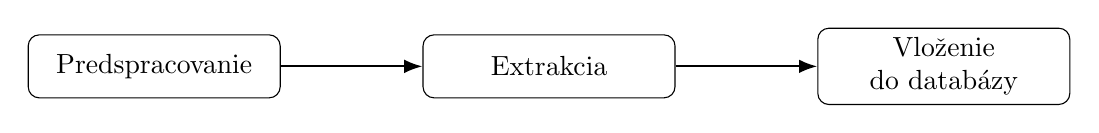
\begin{tikzpicture}[
  node distance=18mm,
  box/.style={draw, rounded corners, minimum height=8mm, minimum width=32mm, align=center},
  arr/.style={-Latex, thick}
]
  \node[box] (pre) {Predspracovanie};
  \node[box, right=of pre] (ext) {Extrakcia};
  \node[box, right=of ext] (db) {Vlo\v{z}enie\\do datab\'azy};

  \draw[arr] (pre) -- (ext);
  \draw[arr] (ext) -- (db);
\end{tikzpicture}
\end{center}


\subsection{Predspracovanie}
V tomto kroku sa PDF dokument načíta, klasifikuje a rozdelí na chunky. Dokument po načítaní
je klasifikovaný pomocou LLM Google Gemini-3-Flash, ktorý určí typ dokumentu (zmluva, zákon, vyhláška, atď.)
a do akého typu práva spadá (ústavné, finančné, občianske, atď.). Pre toto klasifikovanie využívam gemini, kvôli
jeho schopnosti spracovať veľké kontextové okná, rýchlosť ale taktiež pre najlepšie zosumarizovanie textu.
LLM posielam prvých 900,000 tokenov z dokumentu, system prompt, typy dokumentov a právnych odvetví,
a vzor na štruktúrovanú odpoveď.

\

Ako odpoveď dostanem objekt, kde je uložený typ dokumentu \texttt{type\textunderscore category} a typ právneho odvetvia \texttt{type\textunderscore legislation}.
V oboch pripádoch LLM musí uviesť percentuálnu istotu týchto údajov (v rozmedzí 0-100\%). K týmto údajom sa 
dá následne pristupovať ako k Python Dictionary.

\

V ďaľšom kroku prichádza na rozdelenie textu na časti. Využívam funkciu \textbf{RecursiveCharacterTextSplitter}
z balíku \texttt{langchain\textunderscore text\textunderscore splitters}. V otvorenej doméne na extrakciu
schémy rozdeľujem chunky s veľosťou 1200 tokenov a s prekrývaním 200 tokenov. Pri schéme-riadenom extrahovaní
su chunky nastavené na veľkosť 1024 tokenov s prekrývaním 128 tokenov.


\newpage
\subsection{Extrakcia}
Pri extrahovaní entít a vzťahov využívam hybridný prístup na extrakciu na základe štúdie tímu z
apple: \textbf{ODKE+: Ontology-Guided Open-Domain Knowledge Extraction with LLMs}. Kľúčovou vlastnosťou tohto
prístupu je využitie oboch prístupov: štruktúrovaného (schémov-riadené) a neštruktúrovaného (otvorená doména) extrahovania.

\ 

Prečo nie iba schémov-riadené extrahovanie? Navrhnutie výstižnej a bohatej ontológie pre všetky typy práv je
časovo veľmi náročné. S najväčšou pravdepodobnosťou môže nastať situácia,
kde v nejakom dokumente sa vyskytne entita alebo vzťah, ktorý nie je definovaný v ontológii a je kľúčový
pre pochopenie dokumentu. Preto využívam kombináciu oboch prístupov. Je to časovo a cenovo neefektívne riešenie,
avšak prináša najlepšie výsledky. Presnosť extrahovania na základe štúdie dosahuje 98.8\%, čo je pre nás kľúčové.

\

Prečo nie iba extrahovanie v otvorenej doméne? Po tomto prístupe by sme získali veľmi bohatý znalostný graf,
avšak s množstvom nekonzistentných údajov, duplicít a graf by bol chaotický. Kde by boli rozdielne typy entít
ako \texttt{Miesto} a \texttt{Lokácia}, a vznikala by fragmentácia.

\begin{center}
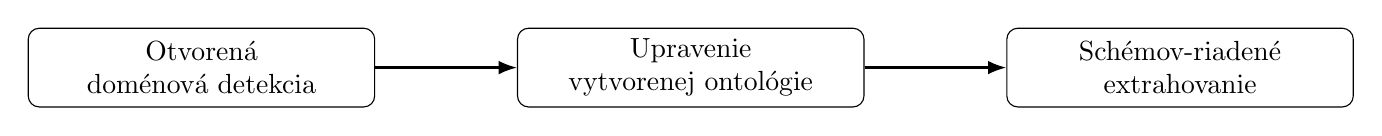
\begin{tikzpicture}[
  node distance=18mm,
  box/.style={draw, rounded corners, minimum height=10mm, minimum width=44mm, align=center},
  arr/.style={-Latex, thick}
]
  \node[box] (det) {Otvoren\'a\\dom\'enov\'a detekcia};
  \node[box, right=of det] (onto) {Upravenie\\vytvorenej ontol\'ogie};
  \node[box, right=of onto] (extr) {Sch\'emov-riaden\'e\\extrahovanie};

  \draw[arr] (det) -- (onto);
  \draw[arr] (onto) -- (extr);
\end{tikzpicture}
\end{center}

\subsubsection{Otvorená doménová detekcia}
Funkcia vytvorí z každého chunku proces, kde všetky procesy bežia paralelne na zníženie času spracovania.
V každom procese je volaný asynchrónne \texttt{agent}. Jehou úlohou je extrahovať každú jednu možnú entitu a vzťah,
ktoré sa nachádzajú v texte chunku. Je to z toho dôvodu, lebo tento krok odhalí nepreddefinované entity a vzťahy,
ktoré môžu byť kľúčové. Vďaka tomuto postupu sa ontológia dynamicky prispôsobí a rozšíri na klasifikovaný 
typ dokumentu a právneho odvetvia. Na tento účel využívam model gpt-4o pre jeho bohaté rozpoznávanie
textu. Následne je vrátená schéma ako zoznamy \texttt{list\textunderscore nodes}
a \texttt{list\textunderscore relationships}.

\subsubsection{Upravenie vytvorenej ontológie}
Vytvorená schéma z predchádzajúceho kroku je poslaná na upravenie. LLM porovná schému s 
preddefinovanou vzorovou ontológiou (sada vytvorených ontológií, ktoré sú konzistentné naprieč slovenským
právom napr. \texttt{Osoba}, \texttt{Zákon}, \texttt{Paragraf}, ...) alebo s už existujúcou schémou znalostného grafu. Tento krok je dôležitý, aby boli údaje
konzistentné, nevytvárali sa sémanticky podobné entity a vzťahy (napr. \texttt{UPRAVUJE} vs \texttt{UPRAVIL})
a nevznikali duplicity. Výstupom tohto kroku je upravená schéma ako zoznamy \texttt{nodes} a \texttt{relationships}.
Využívaný model je gemini-3-flash kvôli jeho dobrým schopnostiam rozmýšľať a odvôvodniť.

\

\subsubsection{Schémov-riadené extrahovanie}
Najprecíznejší krok extrakcie, ktorý zaručuje najvyššiu presnosť a kvalitu extrakcie. Tak isto ako v
otvorenej doméne, aj tu je každý chunk je spracovaný paralelne.
LLM je poskytnutá ontológia z predošlého kroku a na jej základe extrahuje konzistentné entity a vzťahy.
\texttt{Agent} vráti zoznamy \texttt{nodes} a \texttt{relationships}, ktoré sú následne transformované
do \texttt{GraphDocument} objektu.


\ 

Výsledkom je bohatý, konzistentný znalostný graf, ktorý obsahuje všetky relevantné informácie z právnych dokumentov.
Chunky a dokumenty sú pospájané pomocou vzťahu \texttt{PART\textunderscore OF} a chunky s entitami pomocou vzťahu
\texttt{HAS\textunderscore ENTITY}. Medzi entitami sú vzťahy, ktoré sú extrahované z dokumentu.

\

\begin{center}
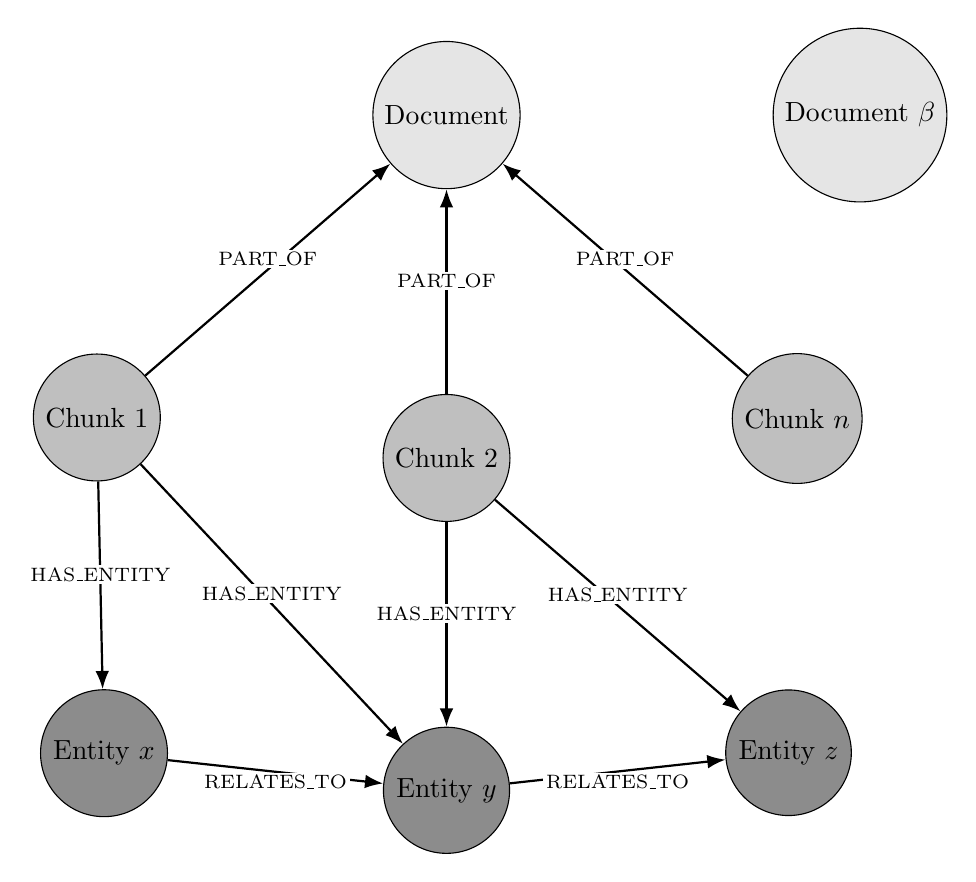
\begin{tikzpicture}[
  node distance=26mm and 32mm,
  doc/.style={circle, draw, fill=gray!20, minimum size=14mm, align=center},
  chunk/.style={circle, draw, fill=gray!50, minimum size=14mm, align=center},
  ent/.style={circle, draw, fill=gray!90, minimum size=14mm, align=center},
  arr/.style={-Latex, thick}
]

  \node[doc] (doc) {Document};
  \node[doc, right=of doc] (doc2) {Document $\beta$};

  \node[chunk, below left=of doc] (c1) {Chunk 1};
  \node[chunk, below=of doc] (c2) {Chunk 2};
  \node[chunk, below right=of doc] (cn) {Chunk $n$};

  \node[ent, below left=of c2] (ex) {Entity $x$};
  \node[ent, below=of c2] (ey) {Entity $y$};
  \node[ent, below right=of c2] (ez) {Entity $z$};

  \draw[arr] (c1) -- node[midway, above, fill=white, inner sep=1pt]{\scriptsize PART\_OF} (doc);
  \draw[arr] (c2) -- node[midway, above, fill=white, inner sep=1pt]{\scriptsize PART\_OF} (doc);
  \draw[arr] (cn) -- node[midway, above, fill=white, inner sep=1pt]{\scriptsize PART\_OF} (doc);

  \draw[arr] (c1) -- node[midway, above, fill=white, inner sep=1pt]{\scriptsize HAS\_ENTITY} (ex);
  \draw[arr] (c1) -- node[midway, above, fill=white, inner sep=1pt]{\scriptsize HAS\_ENTITY} (ey);
  \draw[arr] (c2) -- node[midway, above, fill=white, inner sep=1pt]{\scriptsize HAS\_ENTITY} (ey);
  \draw[arr] (c2) -- node[midway, above, fill=white, inner sep=1pt]{\scriptsize HAS\_ENTITY} (ez);

  \draw[arr] (ex) -- node[midway, below, fill=white, inner sep=1pt]{\scriptsize RELATES\_TO} (ey);
  \draw[arr] (ey) -- node[midway, below, fill=white, inner sep=1pt]{\scriptsize RELATES\_TO} (ez);
\end{tikzpicture}
\end{center}

\newpage
\subsection{Vkladanie do databázy}

\end{document}